\chapter{Analyse}
\label{ch:2}

\section{Anforderungsanalyse}
\label{sec:2.1}

\subsection{Benutzeranforderungen}

Die Applikation erm\"oglicht es dem Benutzer, f\"ur bestimmte 3-D Konstruktionen die Minimalfl\"achen zu berechnen und graphisch darzustellen.\\
Die Applikation gibt nach Starten zun\"achst beispielhafte Einstellungen und Randwerte vor.\\
Der Benutzer kann per Mausklick auf der Benutzeroberfl\"ache zwischen 3 verschiedenen Tabs wechseln.\\
Auf dem ersten Tab ("`Einstellungen"'), das nach Starten des Programmes angezeigt wird, kann der Benutzer die verschiedenen numerischen Parameter (Anzahl der St\"utzstellen in X- und Y Richtung,  Abbruchfehler, maximale Iterationsanzahl, Randfunktionen, Definitionsbereich) in den daf\"ur zust\"andigen Textfeldern \"andern.\\
In den mit "`Grenzen"'  markierten Textfeldern kann der Benutzer Randfunktionen setzen, indem er Funktionen eingibt, f\"ur die die Minimalfl\"achen berechnet werden sollen. Weiterhin kann der Benutzer den Definitionsbereich der Randfunktionen einstellen in den Textfeldern markiert mit "`Definitionsbereich"'.\\
Unter "`Numerische Parameter"'  kann der Benutzer die Parameter f\"ur die Approximation \"andern, die Fehlergrenze, die Anzahl der St\"utzstellen in x- und y- Richtung und die maximale Iterationszahl.
Die maximale Iterationszahl ist die Anzahl an Iterationen, die die Applikation f\"ur die Approximation verwendet, falls die Fehlergrenze nicht vorher unterschritten wird.\\
Der Benutzer kann zu jeder Zeit  mit dem Button "`Quit"' das Programm beenden. \\
Ausserdem kann der Benutzer auch mit einem Mausklick auf "`Einstellungen Speichern"' die gew\"ahlten Einstellungen in einem Dokument speichern und mit einem Klick auf "`Einstellungen Laden"' kann er bereits gespeicherte Einstellungen wiederherstellen.\\
Wenn der Nutzer fertig mit den Einstellungen ist, kann er auf "`Run"'  dr\"ucken, um die Simulation zu starten. \\
Die Applikation checkt die Einstellungen und zeigt im Fehlerfall eine Fehlermeldung an und ansonsten wird die Berechnung gestartet.\\
Geschieht dies, wechselt die Applikation automatisch auf das zweite Tab "`Konsolenausgabe"'.
Weiterhin zeigt die Applikation die Ausgabe der Anwendung an, den Fortschritt, die Iterationszahl und den aktuellen Fehler.\\
Der Fortschritt ist au\" sserdem auf einem Fortschrittsbalken zu sehen.\\
Ist die Berechnung beendet, wechselt die Applikation automatisch auf das dritte Tab "`Anzeige"', wo der Benutzer die fertige 3-D Simulation auf der Zeichenfl\"ache sehen und mithilfe der Maus beliebig drehen kann.\\
Der Benutzer kann dabei jederzeit die Tabs wechseln, auch bevor die Berechnung beendet ist.\\
Wechselt der Benutzer auf das Anzeigetab w\"ahrend die Berechnung l\"auft, dann zeigt die Applikation den derzeitigen Rechenschritt, d.h. den instation\"aren Berechnunungsverlauf an.
Der Benutzer kann auch schon berechnete Minimalfl\"achen (Ergebnisse) speichern oder laden mit einem Mausklick auf den zugeh\"origen Button.\\


%\\
%z.B. L\"osung nichtlinearer Gleichungssysteme resultierend aus Anwendung
%mit Newton's Methode \cite{Heath1998SCA,Kelley2003SNE};
%Problemspezifikation; Weiterverarbeitung der Resultate



\subsection{Anwendungsfallanalyse}

\epsfig{file=Bilder/Top_Level_Use_Cases.eps,width=\textwidth}

\subsubsection{Systemanforderungen}

\textbf{Beenden}
  \begin{itemize}
  \item \textit{Ziel:} Der Nutzer will das Programm beenden.
  \item \textit{Einordnung:} Hauptfunktion
  \item \textit{Vorbedingung:} Die Applikation wurde gestartet.
  \item \textit{Nachbedingung:} Das Programm ist geschlossen. 
  \item \textit{Nachbedingung im Fehlerfall:} 
  \item \textit{Hauptakteure:} Nutzer
  \item \textit{Nebenakteure:}
  \item \textit{Ausl\"oser:} Der Nutzer m\"ochte das Programm beenden.
  \item \textit{Standardablauf:}
  \begin{enumerate}
    \item Der Nutzer klickt auf den Button "Quit".
    \item Die Applikation schlie\ss�t.
  \end{enumerate}
  \end{itemize}

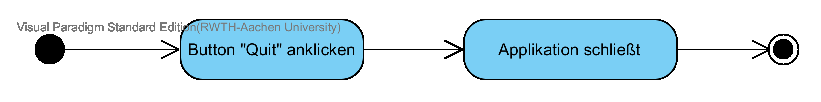
\epsfig{file=Bilder/Beenden1.eps,width=\textwidth}

\textbf{Check Input}
  \begin{itemize}
  \item \textit{Ziel:} Die Applikation will die Gebietsgr\"o\ss e und die numerischen Parameter \"uberpr\"ufen.
  \item \textit{Einordnung:} Hauptfunktion
  \item \textit{Vorbedingung:} Der Nutzer hat auf Run angeklickt.
  \item \textit{Nachbedingung:} Der Use Case "`Check Randfunktionen"' wird gestartet.
  \item \textit{Nachbedingung im Fehlerfall:} Die Applikation zeigt eine Fehlermeldung an und markiert die Stelle, an der sich der Fehler befindet.
  \item \textit{Hauptakteure:} System
  \item \textit{Nebenakteure:}
  \item \textit{Ausl\"oser:} Die Applikation m\"ochte die Gebietsgr\"o\ss e und die numerischen Parameter \"uberpr\"ufen.
  \item \textit{Standardablauf:}
    \begin{enumerate}
    \item Die Applikation pr\"uft, ob die eingegebenen Grenzen der Gebietsgr\"o\ss e g\"ultige double Werte sind.
    \item Die Applikation pr\"uft, ob die obere Grenze xmax gr\"o\ss er als die untere Grenze xmin ist.
    \item Die Applikation pr\"uft, ob die obere Grenze ymax gr\"o\ss er als die untere Grenze ymin ist.
    \item Die Applikation pr\"uft, ob der Abbruchfehler eps gr\"o\ss er 0 und ein double ist.
    \item Die Applikation pr\"uft, ob die maximale Anzahl der Iterationen $max_iteration$, die Anzahl der x-St\"utzstellen n und y-St\"utzstellen m   g\"o\ss er 0 und vom Typ int sind.
  \end{enumerate}
  \item \textit{Verzweigungen:}
    \begin{enumerate}[label=(1a\arabic*)]    
            \item Die Berechnung wird abgebrochen.
	\item Die Applikation zeigt eine Fehlermeldung, falls die Gebietsgr\"o\ss e ung\"ultig ist.(keine Zahl eingegeben oder das Feld leer gelassen)
	\item Das Feld, in dem der Fehler ist, wird markiert.
	\end{enumerate}
	 \begin{enumerate}[label=(2a\arabic*)]    
	 	\item Die Berechnung wird abgebrochen.
		\item Die Applikation zeigt eine Fehlermeldung, falls xmin gr\"o\ss er gleich xmax ist.
		\item Das Feld, in dem der Fehler ist, wird markiert.
	\end{enumerate}
	 \begin{enumerate}[label=(3a\arabic*)]    
	 	\item Die Berechnung wird abgebrochen.
		\item Die Applikation zeigt eine Fehlermeldung, falls ymin gr\"o\ss er gleich ymax ist.\\
		\item Das Feld, in dem der Fehler ist, wird markiert.
	\end{enumerate}
		 \begin{enumerate}[label=(4a\arabic*)]    
		 	\item Die Berechnung wird abgebrochen.
		 \item Die Applikation zeigt eine Fehlermeldung, falls eps ung\"ultig ist.
		 \item Das Feld "`eps edit"' wird markiert.
		 \end{enumerate}
	 \begin{enumerate}[label=(5a\arabic*)]    
	 	\item Die Berechnung wird abgebrochen.
		\item Die Applikation zeigt eine Fehlermeldung, falls ein numerischer Parameter ung\"ultig ist.
		\item Das Feld, in dem der Fehler ist, wird markiert.
    \end{enumerate}
  \end{itemize}

\epsfig{file=Bilder/Check_Input.eps,width=\textwidth}

\textbf{Check Randfunktionen}
  \begin{itemize}
  \item \textit{Ziel:} Das System will die Randfunktionen \"uberpr\"ufen.
  \item \textit{Einordnung:} Hauptfunktion
  \item \textit{Vorbedingung:} Use Case Check Input wurde erfolgreich durchgef\"uhrt.
  \item \textit{Nachbedingung:} Die Berechnung wird durchgef\"uhrt.
  \item \textit{Nachbedingung im Fehlerfall:} Die Applikation zeigt eine Fehlermeldung an und markiert die Stelle, an der sich der Fehler befindet.
  \item \textit{Hauptakteure:} System
  \item \textit{Nebenakteure:}
  \item \textit{Ausl\"oser:} Der Nutzer hat auf 'run' gedr\"uckt und UC Check Input war erfolgreich.
  \item \textit{Standardablauf:}
    \begin{enumerate}
    \item Das System pr\"uft, ob weniger als 2 Variablen vorhanden sind.
    \item Das System pr\"uft, ob die Randfunktionen g\"ultig sind.
  \end{enumerate}
  \item \textit{Verzweigungen:}
    \begin{enumerate}[label=(1a\arabic*)]
	\item Das System zeigt eine Fehlermeldung, falls mehr als 2 Variablen vorhanden sind.
	\item Die Berechnung wird abgebrochen.
	\end{enumerate}
	 \begin{enumerate}[label=(2a\arabic*)]
	\item Das System zeigt eine Fehlermeldung, falls die Randfunktion ung\"ultig ist.
	\item Die Berechnung wird abgebrochen.
    \end{enumerate}
  \end{itemize}

\epsfig{file=Bilder/Check_Randfunktionen.eps,width=\textwidth}

\textbf{Einstellungen laden}
  \begin{itemize}
  \item \textit{Ziel:} Der Nutzer will vorher gespeicherte Einstellungen im .setup Format laden.
  \item \textit{Einordnung:} Hauptfunktion
  \item \textit{Vorbedingung:} Die Applikation wurde gestartet
  \item \textit{Nachbedingung:} Das System l\"adt eine Datei mit den gespeicherten Daten und das MainWindow wird angezeigt.
    \item \textit{Nachbedingung im Fehlerfall:} Nichts wird ver\"andert.
  \item \textit{Hauptakteure:} Nutzer
  \item \textit{Nebenakteure:} System
  \item \textit{Ausl\"oser:} Der Nutzer m\"ochte eine vorher eingestellte gespeicherte Einstellung im .setup Format laden.
    \item \textit{Standardablauf:}
    \begin{enumerate}
    \item Der Nutzer klickt mit der linken Maustaste auf dem Button "Einstellungen laden" an.
    \item Das System zeigt das Dialogfenster an.
    \item Der Nutzer sucht und w\"ahlt einen Ladepfad aus.
    \item Der Nutzer markiert die Datei im .setup Format.
    \item Der Nutzer klickt auf den Button "` \"Offnen"'.
    \item Das System zeigt die gespeicherten Daten im Anzeige Tab an.
  \end{enumerate}
  \item \textit{Verzweigungen:}
    \begin{enumerate}[label=(3\arabic*)]
\item Es befindet sich keine vorher gespeicherte Einstellungsdatei.
    \end{enumerate}
  \end{itemize}

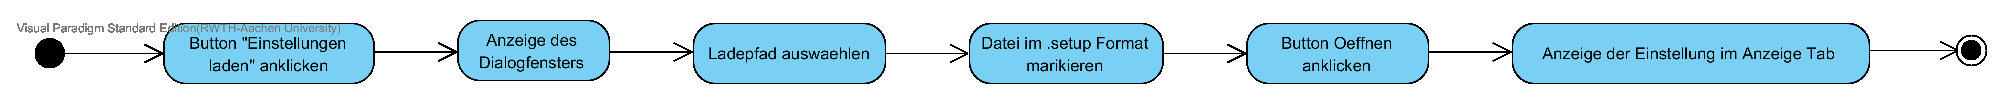
\epsfig{file=Bilder/Einstellungen_laden.eps,width=\textwidth}

\textbf{Einstellungen speichern}
  \begin{itemize}
  \item \textit{Ziel:} Der Nutzer will die eingegebenen Einstellungen speichern.
  \item \textit{Einordnung:} Hauptfunktion
  \item \textit{Vorbedingung:} Die Applikation wurde gestartet.
  \item \textit{Nachbedingung:} Das System erstellt eine .setup Datei mit den gespeicherten Daten und das MainWindow wird angezeigt.
    \item \textit{Nachbedingung im Fehlerfall:}
  \item \textit{Hauptakteure:} Nutzer
  \item \textit{Nebenakteure:} System
  \item \textit{Ausl\"oser:} Der Nutzer m\"ochte die eingegebenen Einstellungen speichern.
    \item \textit{Standardablauf:}
    \begin{enumerate}
    \item Der Nutzer klickt mit der linken Maustaste auf "Einstellungen speichern".
    \item Das System zeigt das Dialogfenster an.
    \item Der Nutzer w\"ahlt den Speicherpfad aus.
    \item Der Nutzer gibt \"uber die Tastatur den Dateinamen ein.
    \item Der Nutzer klickt auf den Button "Speichern".
    \item Das System speichert die eingegebenen  Einstellungen im angegebenen Verzeichnis als .setup Datei
  \end{enumerate}
  \end{itemize}

\epsfig{file=Bilder/Einstellungen_speichern_1.eps,width=\textwidth}

\textbf{Ergebnis laden}
  \begin{itemize}
  \item \textit{Ziel:} Der Nutzer will eine vorher gespeicherte Ergebnisdatei im .surface Format laden.
  \item \textit{Einordnung:} Hauptfunktion
  \item \textit{Vorbedingung:} Die Applikation wurde gestartet
  \item \textit{Nachbedingung:} Das System l\"adt die gespeicherten Ergebnisdaten und zeigt sie im Anzeige Tab an.
    \item \textit{Nachbedingung im Fehlerfall:} Es wird nichts ver\"andert.
  \item \textit{Hauptakteure:} Nutzer
  \item \textit{Nebenakteure:} System
  \item \textit{Ausl\"oser:} Der Nutzer m\"ochte eine vorher gespeicherte Ergebnisdatei im .surface Format laden.
    \item \textit{Standardablauf:}
    \begin{enumerate}
    \item Der Nutzer klickt mit der linken Maustaste auf den Button "Ergebnis laden".
    \item Das System zeigt das Dialogfenster an.
    \item Der Nutzer sucht und w\"ahlt den Ladepfad aus.
    \item Der Nutzer markiert mit der linken Maustaste die .surface Datei.
    \item Der Nutzer klickt mit der linken Maustaste auf den Button \"Offnen.
    \item Das System zeigt die Ergebnisdaten im Anzeige Tab an.   
  \end{enumerate}
  \item \textit{Verzweigungen:}
    \begin{enumerate}[label=(3\arabic*)]
\item Es befindet sich keine vorher gespeicherte Einstellungsdatei.
    \end{enumerate}
  \end{itemize}
\epsfig{file=Bilder/Ergebnis_laden_1.eps,width=\textwidth}
\textbf{Ergebnis speichern}
  \begin{itemize}
  \item \textit{Ziel:} Der Nutzer will die Ergebnisdaten speichern.
  \item \textit{Einordnung:} Hauptfunktion
  \item \textit{Vorbedingung:} Die Applikation wurde gestartet.
  \item \textit{Nachbedingung:} Das System erstellt eine .surface Datei mit den gespeicherten Daten, den numerischen Parametern und der Gebietsgr\"o\ss e. Das MainWindow wird angezeigt.
    \item \textit{Nachbedingung im Fehlerfall:} Das System zeigt eine Fehlermeldung, weil noch keine Berechnung durchgef\"uhrt wurde.
      \item \textit{Hauptakteure:} Nutzer
  \item \textit{Nebenakteure:} System
  \item \textit{Ausl\"oser:} Der Nutzer m\"ochte die Ergebnisdaten speichern.
    \item \textit{Standardablauf:}
    \begin{enumerate}
    \item Der Nutzer klickt mit der linken Maustaste "Ergebnis speichern" an.
    \item Das System pr\"uft, ob eine Berechnung schon durchgef\"uhrt wurde.
    \item Das System zeigt das Dialogfenster an.
    \item Der Nutzer sucht und w\"ahlt einen Pfad aus.
	\item Der Nutzer gibt \"uber die Tastatur den Dateinamen ein.
	\item Der Nutzer klickt auf den Button "Speichern".
	\item Das System speichert die Ergebnisdaten als .surface Datei
  \end{enumerate}
  \item \textit{Verzweigungen:}
    \begin{enumerate}[label=(2\arabic*)]
\item Das System zeigt eine Fehlermeldung an, da zuvor keine Berechnung durchgef\"uhrt wurde.
\item Der UC Ergebnis speichern wird beendet.
    \end{enumerate}
  \end{itemize}
\epsfig{file=Bilder/Einstellungen_speichern_1.eps,width=\textwidth}
\textbf{Gebietsgr\"o\ss e \"Andern}
  \begin{itemize}
  \item \textit{Ziel:} Der Nutzer will einen Wert der Gebietsgr\"o\ss e \"andern.
  \item \textit{Einordnung:} Hauptfunktion
  \item \textit{Vorbedingung:} Die Applikation wurde gestartet und der Tab 'Einstellungen' im MainWindow wird angezeigt.
  \item \textit{Nachbedingung:} Die Gebietsgr\"o\ss e wurde ver\"andert.
  \item \textit{Nachbedingung im Fehlerfall:} 
  \item \textit{Hauptakteure:} Nutzer
  \item \textit{Nebenakteure:} System
  \item \textit{Ausl\"oser:} Der Nutzer m\"ochte einen Wert der Gebietsgr\"o\ss e \"andern.
  \item \textit{Standardablauf:}
    \begin{enumerate}
    \item Der Nutzer klickt mit der linken Maustaste auf beliebiges Feld der Gebietsgr\"o\ss e.
    \item Der Nutzer gibt \"uber die Tastatur den neuen Wert der Gebietsgr\"o\ss e ein.
  \end{enumerate}
  \end{itemize}

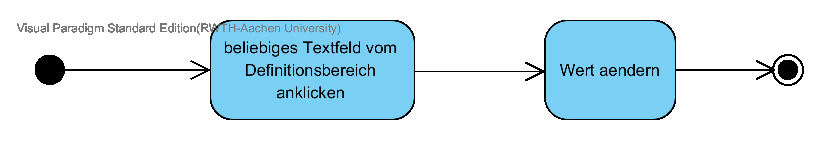
\epsfig{file=Bilder/Gebietsgroesse_aendern1.eps,width=\textwidth}
\textbf{Numerische Parameter \"Andern}
  \begin{itemize}
  \item \textit{Ziel:} Der Nutzer will einen  numerischen Parameter \"andern.
  \item \textit{Einordnung:} Hauptfunktion
  \item \textit{Vorbedingung:} Die Applikation wurde gestartet und der Tab 'Setting' im MainWindow wird angezeigt.
  \item \textit{Nachbedingung:} Der numerische Parameter wurde ver\"andert.
  \item \textit{Nachbedingung im Fehlerfall:} 
  \item \textit{Hauptakteure:} Nutzer
  \item \textit{Nebenakteure:} System
  \item \textit{Ausl\"oser:} Der Nutzer m\"ochte einen  numerischen Parameter \"andern.
  \item \textit{Standardablauf:}
    \begin{enumerate}
    \item Der Nutzer klickt mit der linken Maustaste auf beliebiges Feld der numerischen Parameter. 
    \item Der Nutzer gibt \"uber die Tastatur den neuen numerischen Wert ein.
  \end{enumerate}
  \end{itemize}
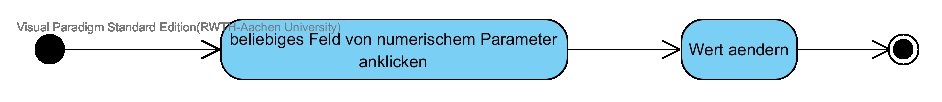
\epsfig{file=Bilder/Numerische_Parameter_aendern.eps,width=\textwidth}
\textbf{Randfunktionen \"Andern}
  \begin{itemize}
  \item \textit{Ziel:} Der Nutzer will eine Randfunktion \"andern.
  \item \textit{Einordnung:} Hauptfunktion
  \item \textit{Vorbedingung:} Die Applikation wurde gestartet und der Tab 'Setting' im MainWindow wird angezeigt.
  \item \textit{Nachbedingung:} Die Randfunktion wurde ver\"andert.
  \item \textit{Nachbedingung im Fehlerfall:}  
  \item \textit{Hauptakteure:} Nutzer
  \item \textit{Nebenakteure:} System
  \item \textit{Ausl\"oser:} Der Nutzer m\"ochte eine Randfunktion \"andern.
  \item \textit{Standardablauf:}
    \begin{enumerate}
    \item Der Nutzer klickt mit der linken Maustaste auf beliebiges Feld der Randfunktionen an.
    \item Der Nutzer gibt \"uber die Tastatur die neue Randfunktion ein. 
  \end{enumerate}
  \end{itemize}
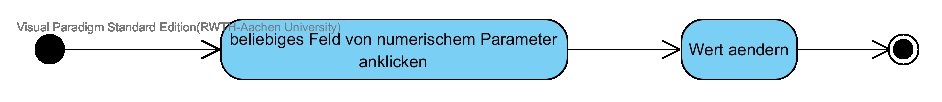
\epsfig{file=Bilder/Numerische_Parameter_aendern.eps,width=\textwidth}
\textbf{run}
  \begin{itemize}
  \item \textit{Ziel:} Der Nutzer will die Berechnung der Minimalfl\"ache durchf\"uhren und anzeigen.
  \item \textit{Einordnung:} Hauptfunktion
  \item \textit{Vorbedingung:} Die Applikation wurde gestartet, alle numerische Parameter, Randfunktionen und Gebietsgr\"o\ss e sind eingegeben.
  \item \textit{Nachbedingung:} Die Applikation zeigt die berechneten Minimalfl\"achen im Tab "`Anzeige"' an.
    \item \textit{Nachbedingung im Fehlerfall:} Es wird eine Fehlermeldung angezeigt.
  \item \textit{Hauptakteure:} Nutzer
  \item \textit{Nebenakteure:} System
  \item \textit{Ausl\"oser:} Der Nutzer will die Berechnung starten.
    \item \textit{Standardablauf:}
    \begin{enumerate}
    \item Der Nutzer klickt mit der linken Maustaste auf den Button 'Run'.
    \item UC "`Check Input"'
    \item UC "`Check Randfunktionen"'
    \item Die Applikation wechselt den Tab auf "`Konsolenausgabe"'.
    \item Die Applikation startet mit den gegeben Einstellungen die Berechnung der Minimalf\"achen.
    \item Die Applikation zeigt den Fortschritt der Berechnung auf der Benutzeroberfl\"ache an.
    \item Die Applikation schliesst die Berechnung ab.
    \item Die Applikation wechselt den Tab auf "`Anzeige"'
    \item Die Applikation zeigt die berechnete Minimalfl\"ache an.
  \end{enumerate}
  \item \textit{Verzweigungen:}
      \begin{enumerate}[label=(2a\arabic*)]
  \item Der UC "`Check Input"' ist fehlerhaft, die Applikation zeigt eine Fehlermeldung an und stoppt die Berechnung.
      \end{enumerate}
    \begin{enumerate}[label=(3a\arabic*)]
  \item Der UC "`Check Randfunktionen"' ist fehlerhaft, die Applikation zeigt eine Fehlermeldung an und stoppt die Berechnung.
    \end{enumerate}
    \begin{enumerate}[label=(7a\arabic*)]
    \item Die Berechnung ist nicht konvergiert, die Applikation zeigt auf der "`Konsolenausgabe"' eine Fehlermeldung an.
     \item Die Applikation wechselt den Tab auf "`Anzeige"'
     \item Die Applikation zeigt die nicht vollst\"andig berechnete Minimalfl\"ache an.
        \end{enumerate}
  \end{itemize}
\epsfig{file=Bilder/Run1.eps,width=\textwidth}
\textbf{Tab wechseln}
  \begin{itemize}
  \item \textit{Ziel:} Der Nutzer will zu einem anderen Tab wechseln.
  \item \textit{Einordnung:} Hauptfunktion
  \item \textit{Vorbedingung:} Die Applikation wurde erfolgreich gestartet.
  \item \textit{Nachbedingung:} Die Applikation zeigt den neuen Tab an.
  \item \textit{Nachbedingung im Fehlerfall:} 
  \item \textit{Hauptakteure:} Nutzer
  \item \textit{Nebenakteure:} System
  \item \textit{Ausl\"oser:} Der Nutzer m\"ochte auf einen anderen Tab wechseln.
  \item \textit{Standardablauf:}
    \begin{enumerate}
     \item Der Nutzer klickt mit der linken Maustaste auf den gew\"unschten Tab.
    \item Die Applikation wechselt den Tab und zeigt den ausgew\"ahlten Tab an.
  \end{enumerate}
  \end{itemize}
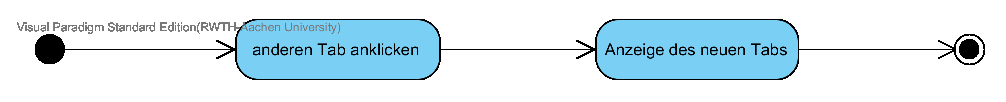
\epsfig{file=Bilder/Tab_wechseln1.eps,width=\textwidth}


\subsection{Funktionale Anforderung}
\begin{itemize}
\item Anzeigen einer Benutzeroberfl\"ache
\item Speichern der Einstellungen
\item Laden der Einstellungen
\item Speichern der Ergebnisse
\item Laden der Ergebnisse
\item M\"oglicher Wechsel zwischen drei Tabs. Funktionen des ersten Tabs (Einstellungen):
	\begin{enumerate}
	\item Eingabe der Anzahl der St\"utzstellen in X- und Y-Richtung
	\item Eingabe der Randfunktionen
	\item Eingabe des Abbruchfehlers
	\item Eingabe der Anzahl der maximalen Iterationen
	\item \"Anderung des Gebietes
	\item Run Button
	\item Quit Button
	\end{enumerate}
\item Funktionen des zweiten Tabs (Konsolenausgabe):
	\begin{enumerate}
	\item Anzeigen des Fortschrittes
	\item Anzeigen von Fehlermeldungen
	\end{enumerate}
\item Funktionen des dritten Tabs (Anzeige):
	\begin{enumerate}
	\item Graphische Darstellung der berechneten Minimalfl\"achen
	\item Plot: variabler viewpoint
	\item Instation\"are Anzeige des derzeitigen Ergebnisses w\"ahrend der Berechnung
	\end{enumerate}
\item Test auf G\"ultigkeit des Gebietsbereiches
\item Test auf ganze Zahl der Anzahl der St\"utzstellen.
\end{itemize}
\subsection{Nicht Funktionale Anforderung}
\begin{itemize}
\item Eingabe der Zahlen durch Tastatur
\item Skalierung des Hauptfensters bei unterschiedlichen Aufl\"osungen.
		\item Skalierung des Hauptfensters bei unterschiedlichen Aufl\"osungen
		\item Erzeugung von korrekten Ergebnissen
		\item Intuitive Bedienbarkeit
		\item Plattformunabh\"angig
		\item Effiziente Berechnung
\end{itemize}


\section{Begriffsanalyse}

\epsfig{file=Bilder/Begriffsmodel.eps,width=\textwidth}



\noindent \textbf{Klassenkadidaten} 
\begin{itemize}
	\item \textbf{Diskretisierung}
	\item \textbf{Eingabebereich}
	\item \textbf{Ausgabebereich}
	\item \textbf{Main Window}
	\item Textfeld f\"ur Eingabe
	\item Button
	\item Radiobutton
	\item Dialogfenster
	\item Fehlermeldung(durch main implementiert)
	\item Berechnungsparameter
	\item Randwert
	\item Gebietsgr\"o\ss e
\end{itemize}





